\chapter{Análisis}

\section{Análisis de requisitos}

El primer paso en el análisis de un desarrollo software es identificar los requisitos funcionales y no funcionales. Estos requisitos son los que deberá garantizar el producto final y son generados a partir de las entrevistas con el cliente y los objetivos marcados para el software.

\bigskip
Nuestra metodología es ágil basada en iteraciones incrementales por lo que los requisitos son analizados en cada iteración, pudiendo ser modificados según las necesidades.


\subsection{Requisitos funcionales}

Los requisitos funcionales son las características que debe satisfacer el sistema, es decir, todas aquellas funciones que debe cumplir el producto final:

\begin{itemize}
	\item \textbf{RF-1.} Conectarse con un servidor INDI.
	\item \textbf{RF-2.} Gestionar conexiones (crear, editar y borrar).
	\item \textbf{RF-3.} Listar todos los dispositivos de una conexión INDI.
	\item \textbf{RF-4.} Listar todas las propiedades de un dispositivo INDI.
	\item \textbf{RF-5.} Tener más de una conexión INDI simultáneamente.
	\item \textbf{RF-6.} Mostrar un log para cada conexión.
	\item \textbf{RF-7.} Agrupar las propiedades por grupos.
	\item \textbf{RF-8.} Editar las propiedades INDI:
		\begin{itemize}
			\item \textbf{RF-8.1.} Propiedad Blob.
			\item \textbf{RF-8.2.} Propiedad Switch.
			\item \textbf{RF-8.3.} Propiedad Number.
			\item \textbf{RF-8.4.} Propiedad Text.
			\item \textbf{RF-8.5.} Propiedad Light.
		\end{itemize}
\end{itemize}

\subsection{Requisitos no funcionales}

Los requerimientos no funcionales, como su nombre sugiere, son aquellos requerimientos que no se refieren directamente a las funciones específicas que proporciona el sistema, sino a las propiedades emergentes de éste:

\begin{itemize}
  \item \textbf{RN-1.} Las interfaces deben seguir las recomendaciones de diseño establecidas por Android.
  \item \textbf{RN-2.} Se deben usar las clases y elementos de interfaz recomendados para la última versión de Android y usar las bibliotecas de compatibilidad.
  \item \textbf{RN-3.} Controlar la hebra principal para no sobre cargarla, creando nuevas hebras en paralelo mejorando así el rendimiento.
  \item \textbf{RN-4.} Crear interfaces específicas para las propiedades genéricas de INDI y para dispositivos conocidos.
  \item \textbf{RN-5.} Utilizar licencias libres para publicar el proyecto como Software libre
  \item \textbf{RN-6.} Adaptar la aplicación a distintos tamaños de pantalla.
  \item \textbf{RN-7.} Diseñar el software para facilitar la extensibilidad de las vistas de dispositivos y propiedades.
  \item \textbf{RN-8.} Internacionalización de la aplicación: Mínimo inglés y castellano.
\end{itemize}

\section{Casos de uso}

Un caso de uso es una descripción de los pasos o las actividades que deberán realizarse para llevar a cabo algún proceso. Los personajes o entidades que participarán en un caso de uso se denominan actores

\subsection{Descripción de actores}

\begin{itemize}
  \item \textbf{Ac-1.} Usuario.
  \begin{itemize}
   \item Descripción: Persona que utilizará la aplicación.
   \item Características: Es el usuario estándar de una aplicación.
   \item Relaciones: Ninguna.
   \item Atributos: Ninguno.
   \item Comentarios: El usuario no tiene ningún conocimiento previo.
  \end{itemize}
\end{itemize}

\subsection{Descripción casos de uso}

\begin{itemize}
  \item \textbf{CU-1.} Añadir una conexión.
  \begin{itemize}
    \item Actores: Usuario.
    \item Tipo: Primario, esencial.
    \item Referencias:
    \item Precondición:
    \item Postcondición: La nueva conexión será añadida a la lista y guardada.
    \item Autor: \autor.
    \item Versión: 1.0.
    \item Propósito: Añadir una nueva conexión.
    \item Resumen: El usuario rellenará una serie de campos y marcará unas opciones para añadir una nueva conexión a la lista.
    \end{itemize}
    \begin{table}[!ht]
      \begin{center}
	\begin{tabular}{|l|l|l|l|}
	  \hline
	  \multicolumn{4}{|c|}{{\bf Curso normal}}
	  \\ \hline
	  \multicolumn{2}{|c|}{{\bf Actor}} & \multicolumn{2}{c|}{{\bf Sistema}}
	  \\ \hline
	  {\it 1} & 
	  \begin{tabular}[c]{@{}l@{}}
	    Usuario: Pulsa el botón para\\
	    añadir una nueva conexión.\\
	  \end{tabular} &
	  &
	  \\ \hline
	  &
	  &
	  {\it 2} &
	  \begin{tabular}[c]{@{}l@{}}
	    El sistema muestra el formulario\\
	    para añadir nuevas conexiones. \\
	  \end{tabular}
	  \\ \hline
	  {\it 3} & 
	  \begin{tabular}[c]{@{}l@{}}
	    Usuario: Rellena los campos del \\
	    formulario, marca las opciones  \\
	    y pulsa en el botón de añadir.   \\
	  \end{tabular} &
	  &
	  \\ \hline
	  &
	  &
	  {\it 4} &
	  \begin{tabular}[c]{@{}l@{}}
	    El sistema almacena la conexión\\
	    y la añade a la lista de conexiones.\\
	  \end{tabular}
	  \\ \hline
	\end{tabular}
	\caption{CU-1. Añadir nueva conexión.}
	\label{table:cu_1}
      \end{center}
    \end{table}
    \newpage
    \item \textbf{CU-2.} Editar una conexión.
  \begin{itemize}
    \item Actores: Usuario.
    \item Tipo: Primario, esencial.
    \item Referencias:
    \item Precondición: La conexión debe existir y estar en estado ``desconectada''.
    \item Postcondición: La conexión sera editada y guardada.
    \item Autor: \autor.
    \item Versión: 1.0.
    \item Propósito: Editar una conexión existente.
    \item Resumen: El usuario rellenará una serie de campos y marcará unas opciones para editar la conexión.
    \end{itemize}
    \begin{table}[!ht]
      \begin{center}
	\begin{tabular}{|l|l|l|l|}
	  \hline
	  \multicolumn{4}{|c|}{{\bf Curso normal}}
	  \\ \hline
	  \multicolumn{2}{|c|}{{\bf Actor}} & \multicolumn{2}{c|}{{\bf Sistema}}
	  \\ \hline
	  {\it 1} & 
	  \begin{tabular}[c]{@{}l@{}}
	    Usuario: Pulsa el botón para\\
	    desplegar el menú lateral.\\
	  \end{tabular} &
	  &
	  \\ \hline
	  &
	  &
	  {\it 2} &
	  \begin{tabular}[c]{@{}l@{}}
	    El sistema muestra el menú lateral\\
	    con las conexiones, su estado y sus \\
	    dispositivos.\\
	  \end{tabular}
	  \\ \hline
	  {\it 3} & 
	  \begin{tabular}[c]{@{}l@{}}
	    Usuario: Pulsa el botón editar\\
	    para una conexión concreta.\\
	  \end{tabular} &
	  &
	  \\ \hline
	  &
	  &
	  {\it 4} &
	  \begin{tabular}[c]{@{}l@{}}
	    El sistema muestra el formulario\\
	    para la edición de una conexión. \\
	  \end{tabular}
	  \\ \hline
	  {\it 5} & 
	  \begin{tabular}[c]{@{}l@{}}
	    Usuario: edita los campos del \\
	    formulario, marca las opciones  \\
	    y pulsa en el botón de editar.   \\
	  \end{tabular} &
	  &
	  \\ \hline
	  &
	  &
	  {\it 6} &
	  \begin{tabular}[c]{@{}l@{}}
	    El sistema almacena la conexión\\
	  \end{tabular}
	  \\ \hline
	\end{tabular}
	\caption{CU-2. Editar una conexión.}
	\label{table:cu_2}
      \end{center}
    \end{table}

    \newpage
     \item \textbf{CU-3.} Borrar conexiones.
  \begin{itemize}
    \item Actores: Usuario.
    \item Tipo: Primario, esencial.
    \item Referencias:
    \item Precondición: Las conexiones deben existir.
    \item Postcondición: Las conexiones serán borradas.
    \item Autor: \autor.
    \item Versión: 1.0.
    \item Propósito: Borrar conexiones.
    \item Resumen: El usuario seleccionará de entre las conexiones disponibles, una selección para que sean borradas.
    \end{itemize}
    \begin{table}[!ht]
      \begin{center}
	\begin{tabular}{|l|l|l|l|}
	  \hline
	  \multicolumn{4}{|c|}{{\bf Curso normal}}
	  \\ \hline
	  \multicolumn{2}{|c|}{{\bf Actor}} & \multicolumn{2}{c|}{{\bf Sistema}}
	  \\ \hline
	  {\it 1} & 
	  \begin{tabular}[c]{@{}l@{}}
	    Usuario: Pulsa el botón para\\
	    desplegar el menú superior derecho.\\
	  \end{tabular} &
	  &
	  \\ \hline
	  &
	  &
	  {\it 2} &
	  \begin{tabular}[c]{@{}l@{}}
	    El sistema muestra el menú superior.\\
	  \end{tabular}
	  \\ \hline
	  {\it 3} & 
	  \begin{tabular}[c]{@{}l@{}}
	    Usuario: Pulsa el botón para\\
	    borrar conexiones.\\
	  \end{tabular} &
	  &
	  \\ \hline
	  &
	  &
	  {\it 4} &
	  \begin{tabular}[c]{@{}l@{}}
	    El sistema muestra el formulario\\
	    con una lista de todas las conexiones \\
	  \end{tabular}
	  \\ \hline
	  {\it 5} & 
	  \begin{tabular}[c]{@{}l@{}}
	    Usuario: selecciona aquellas conexiones\\
	    que desee borrar.\\
	  \end{tabular} &
	  &
	  \\ \hline
	  &
	  &
	  {\it 6} &
	  \begin{tabular}[c]{@{}l@{}}
	    El sistema Borra las conexiones\\ 
	    seleccionadas\\
	  \end{tabular}
	  \\ \hline
	\end{tabular}
	\caption{CU-3. Borrar conexiones.}
	\label{table:cu_3}
      \end{center}
    \end{table}

    \newpage
    \item \textbf{CU-4.} Editar los ajustes.
  \begin{itemize}
    \item Actores: Usuario.
    \item Tipo: Opcional, esencial.
    \item Referencias:
    \item Precondición:
    \item Postcondición: Los ajustes serán guardados.
    \item Autor: \autor.
    \item Versión: 1.0.
    \item Propósito: Editar los ajustes.
    \item Resumen: El usuario establecerá las distintas configuraciones.
    \end{itemize}
    \begin{table}[!ht]
      \begin{center}
	\begin{tabular}{|l|l|l|l|}
	  \hline
	  \multicolumn{4}{|c|}{{\bf Curso normal}}
	  \\ \hline
	  \multicolumn{2}{|c|}{{\bf Actor}} & \multicolumn{2}{c|}{{\bf Sistema}}
	  \\ \hline
	  {\it 1} & 
	  \begin{tabular}[c]{@{}l@{}}
	    Usuario: Pulsa el botón para\\
	    desplegar el menú superior derecho.\\
	  \end{tabular} &
	  &
	  \\ \hline
	  &
	  &
	  {\it 2} &
	  \begin{tabular}[c]{@{}l@{}}
	    El sistema muestra el menú superior.\\
	  \end{tabular}
	  \\ \hline
	  {\it 3} & 
	  \begin{tabular}[c]{@{}l@{}}
	    Usuario: Pulsa el botón para\\
	    ver los ajustes.\\
	  \end{tabular} &
	  &
	  \\ \hline
	  &
	  &
	  {\it 4} &
	  \begin{tabular}[c]{@{}l@{}}
	    El sistema muestra la pantalla cin\\
	    con una lista de ajustes y su estado.\\
	  \end{tabular}
	  \\ \hline
	  {\it 5} & 
	  \begin{tabular}[c]{@{}l@{}}
	    Usuario: editada los ajustes que\\ 
	    considere.\\
	  \end{tabular} &
	  &
	  \\ \hline
	  &
	  &
	  {\it 6} &
	  \begin{tabular}[c]{@{}l@{}}
	    El sistema guarda el estado de\\
	    cada configuración.
	  \end{tabular}
	  \\ \hline
	\end{tabular}
	\caption{CU-4. Editar los ajustes.}
	\label{table:cu_4}
      \end{center}
    \end{table}

    \newpage
    \item \textbf{CU-5.} Conectarse a un servidor.
  \begin{itemize}
    \item Actores: Usuario.
    \item Tipo: Primario, esencial.
    \item Referencias:
    \item Precondición: La conexión debe haber sido añadida previamente. La conexión debe estar desconectada.
    \item Postcondición: Se añaden los dispositivos de la conexión a la lista (si los hubiese).
    \item Autor: \autor.
    \item Versión: 1.0.
    \item Propósito: Conectarse a un servidor.
    \item Resumen: El usuario se conectará a un servidor.
    \end{itemize}
    \begin{table}[!ht]
      \begin{center}
	\begin{tabular}{|l|l|l|l|}
	  \hline
	  \multicolumn{4}{|c|}{{\bf Curso normal}}
	  \\ \hline
	  \multicolumn{2}{|c|}{{\bf Actor}} & \multicolumn{2}{c|}{{\bf Sistema}}
	  \\ \hline
	  {\it 1} & 
	  \begin{tabular}[c]{@{}l@{}}
	    Usuario: Pulsa el botón para\\
	    desplegar el menú lateral izquierdo.\\
	  \end{tabular} &
	  &
	  \\ \hline
	  &
	  &
	  {\it 2} &
	  \begin{tabular}[c]{@{}l@{}}
	    El sistema muestra el menú lateral\\
	    izquierdo con la lista de conexiones \\
	    y dispositivos.\\
	  \end{tabular}
	  \\ \hline
	  {\it 3} & 
	  \begin{tabular}[c]{@{}l@{}}
	    Usuario: Pulsa el botón para\\
	    conectarse.\\
	  \end{tabular} &
	  &
	  \\ \hline
	  &
	  &
	  {\it 4a} &
	  \begin{tabular}[c]{@{}l@{}}
	    El sistema esconde el menú lateral y\\
	    realiza la conexión. A partir de ahora \\
	    la conexión se mantiene en segundo plano\\
	    para refrescar los dispositivos añadidos \\
	    o borrados que serán listados al desplegar\\
	    el menú lateral izquierdo.
	  \end{tabular}
	  \\ \hline
	\end{tabular}
	\caption{CU-4. Conectarse a un servidor.}
	\label{table:cu_5}
      \end{center}
    \end{table}
    \begin{table}[!ht]
      \begin{center}
	\begin{tabular}{|l|l|}
	  \hline
	  \multicolumn{2}{|c|}{{\bf Curso alterno}}
	  \\ \hline
	  {\it 4b} &
	  \begin{tabular}[c]{@{}l@{}}
	    Si el servidor no responde, o los datos de la conexión no son\\
	    correctos, el sistema muestra una alerta para informar al \\
	    usuario.\\
	  \end{tabular}\\
	  \hline
	\end{tabular}
	\caption{Curso alterno de CU-5. Conectarse a un servidor.}
	\label{table:ca_cu_5}
      \end{center}
    \end{table}

    \newpage
    \item \textbf{CU-6.} Desconectarse de un servidor.
  \begin{itemize}
    \item Actores: Usuario.
    \item Tipo: Primario, esencial.
    \item Referencias:
    \item Precondición: La conexión debe haber sido añadida previamente. La conexión debe estar conectada.
    \item Postcondición: Se borran de la lista los dispositivos (si los hubiera).
    \item Autor: \autor.
    \item Versión: 1.0.
    \item Propósito: Desconectarse de un servidor.
    \item Resumen: El usuario se desconecta de un servidor.
    \end{itemize}
    \begin{table}[!ht]
      \begin{center}
	\begin{tabular}{|l|l|l|l|}
	  \hline
	  \multicolumn{4}{|c|}{{\bf Curso normal}}
	  \\ \hline
	  \multicolumn{2}{|c|}{{\bf Actor}} & \multicolumn{2}{c|}{{\bf Sistema}}
	  \\ \hline
	  {\it 1} & 
	  \begin{tabular}[c]{@{}l@{}}
	    Usuario: Pulsa el botón para\\
	    desplegar el menú lateral izquierdo.\\
	  \end{tabular} &
	  &
	  \\ \hline
	  &
	  &
	  {\it 2} &
	  \begin{tabular}[c]{@{}l@{}}
	    El sistema muestra el menú lateral\\
	    izquierdo con la lista de conexiones \\
	    y dispositivos.\\
	  \end{tabular}
	  \\ \hline
	  {\it 3} & 
	  \begin{tabular}[c]{@{}l@{}}
	    Usuario: Pulsa el botón para\\
	    desconectarse.\\
	  \end{tabular} &
	  &
	  \\ \hline
	  &
	  &
	  {\it 4} &
	  \begin{tabular}[c]{@{}l@{}}
	    El sistema esconde el menú lateral y\\
	    realiza la desconexión. .
	  \end{tabular}
	  \\ \hline
	\end{tabular}
	\caption{CU-6. Desconectarse de un servidor.}
	\label{table:cu_6}
      \end{center}
    \end{table}

    \newpage
    \item \textbf{CU-7.} Salir de la aplicación.
  \begin{itemize}
    \item Actores: Usuario.
    \item Tipo: Secundario, esencial.
    \item Referencias:
    \item Precondición: La aplicación debe estar iniciada.
    \item Postcondición: Se cierran todas las conexiones, hebras y procesos liberando todos los recursos de la aplicación.
    \item Autor: \autor.
    \item Versión: 1.0.
    \item Propósito: Salir de la aplicación.
    \item Resumen: El usuario cierra la aplicación explícitamente.
    \end{itemize}
    \begin{table}[!ht]
      \begin{center}
	\begin{tabular}{|l|l|l|l|}
	  \hline
	  \multicolumn{4}{|c|}{{\bf Curso normal}}
	  \\ \hline
	  \multicolumn{2}{|c|}{{\bf Actor}} & \multicolumn{2}{c|}{{\bf Sistema}}
	  \\ \hline
	  {\it 1} & 
	  \begin{tabular}[c]{@{}l@{}}
	    Usuario: Pulsa el botón para\\
	    desplegar el menú superior derecho.\\
	  \end{tabular} &
	  &
	  \\ \hline
	  &
	  &
	  {\it 2} &
	  \begin{tabular}[c]{@{}l@{}}
	    El sistema muestra el menú superior.\\
	  \end{tabular}
	  \\ \hline
	  {\it 3} & 
	  \begin{tabular}[c]{@{}l@{}}
	    Usuario: Pulsa el botón salir.\\
	  \end{tabular} &
	  &
	  \\ \hline
	  &
	  &
	  {\it 4} &
	  \begin{tabular}[c]{@{}l@{}}
	    El sistema comprueba cada conexión\\ 
	    y se desconecta de todas, cerrando\\
	    todas las hebras. Después cierra la\\ 
	    aplicación.
	  \end{tabular}
	  \\ \hline
	\end{tabular}
	\caption{CU-7. Salir de la aplicación.}
	\label{table:cu_7}
      \end{center}
    \end{table}

    \newpage
    \item \textbf{CU-8.} Mostrar dispositivo.
  \begin{itemize}
    \item Actores: Usuario.
    \item Tipo: Primario, esencial.
    \item Referencias:
    \item Precondición: La conexión debe haber sido añadida previamente. La conexión debe estar conectada.
    \item Postcondición: Se listan todas las propiedades del dispositivo. Cualquier cambio en las propiedades será mostrado en la lista en tiempo real.
    \item Autor: \autor.
    \item Versión: 1.0.
    \item Propósito: Mostrar las propiedades de un dispositivo.
    \item Resumen: El usuario selecciona un dispositivo para mostrar la lista de sus propiedades.
    \end{itemize}
    \begin{table}[!ht]
      \begin{center}
	\begin{tabular}{|l|l|l|l|}
	  \hline
	  \multicolumn{4}{|c|}{{\bf Curso normal}}
	  \\ \hline
	  \multicolumn{2}{|c|}{{\bf Actor}} & \multicolumn{2}{c|}{{\bf Sistema}}
	  \\ \hline
	  {\it 1} & 
	  \begin{tabular}[c]{@{}l@{}}
	    Usuario: Pulsa el botón para\\
	    desplegar el menú lateral izquierdo.\\
	  \end{tabular} &
	  &
	  \\ \hline
	  &
	  &
	  {\it 2} &
	  \begin{tabular}[c]{@{}l@{}}
	    El sistema muestra el menú lateral\\
	    izquierdo con la lista de conexiones \\
	    y dispositivos.\\
	  \end{tabular}
	  \\ \hline
	  {\it 3} & 
	  \begin{tabular}[c]{@{}l@{}}
	    Usuario: Pulsa sobre el dispositivo\\
	    deseado.\\
	  \end{tabular} &
	  &
	  \\ \hline
	  &
	  &
	  {\it 4} &
	  \begin{tabular}[c]{@{}l@{}}
	    El sistema esconde el menú lateral y\\
	    y muestra una pantalla tabulada con\\
	    todas las vistas especiales que tenga\\
	    el dispositivo (si las tiene) más la\\
	    vista por defecto con la lista de \\
	    de propiedades y la ayuda general de\\
	    la aplicación.
	  \end{tabular}
	  \\ \hline
	\end{tabular}
	\caption{CU-8. Mostrar dispositivo.}
	\label{table:cu_8}
      \end{center}
    \end{table}

    \newpage
    \item \textbf{CU-9.} Cambiar vista de dispositivo.
  \begin{itemize}
    \item Actores: Usuario.
    \item Tipo: Primario, esencial.
    \item Referencias:
    \item Precondición: El usuario debe haber seleccionado un dispositivo (CU-8).
    \item Postcondición:
    \item Autor: \autor.
    \item Versión: 1.0.
    \item Propósito: Cambiar entre las vistas de un dispositivo.
    \item Resumen: El usuario cambia de vista de un dispositivo entre las disponibles.
    \end{itemize}
    \begin{table}[!ht]
      \begin{center}
	\begin{tabular}{|l|l|l|l|}
	  \hline
	  \multicolumn{4}{|c|}{{\bf Curso normal}}
	  \\ \hline
	  \multicolumn{2}{|c|}{{\bf Actor}} & \multicolumn{2}{c|}{{\bf Sistema}}
	  \\ \hline
	  {\it 1} & 
	  \begin{tabular}[c]{@{}l@{}}
	    Usuario: Pulsa sobre el nombre\\
	    de la pestaña correspondiente o \\
	    desliza el dedo por la pantalla.\\
	  \end{tabular} &
	  &
	  \\ \hline
	  &
	  &
	  {\it 2} &
	  \begin{tabular}[c]{@{}l@{}}
	    El sistema muestra la vista correspondiente.\\
	  \end{tabular}
	  \\ \hline
	\end{tabular}
	\caption{CU-9. Cambiar vista de dispositivo.}
	\label{table:cu_9}
      \end{center}
    \end{table}

    \newpage
    \item \textbf{CU-10.} Editar propiedad \textit{text}.
  \begin{itemize}
    \item Actores: Usuario.
    \item Tipo: Primario, esencial.
    \item Referencias:
    \item Precondición: El usuario debe haber seleccionado un dispositivo (CU-8).
    \item Postcondición: La propiedad es editada y enviada al servidor.
    \item Autor: \autor.
    \item Versión: 1.0.
    \item Propósito: Editar una propiedad \textit{text}.
    \item Resumen: El usuario pulsará sobre una propiedad \textit{text} para editarla.
    \end{itemize}
    \begin{table}[!ht]
      \begin{center}
	\begin{tabular}{|l|l|l|l|}
	  \hline
	  \multicolumn{4}{|c|}{{\bf Curso normal}}
	  \\ \hline
	  \multicolumn{2}{|c|}{{\bf Actor}} & \multicolumn{2}{c|}{{\bf Sistema}}
	  \\ \hline
	  {\it 1} & 
	  \begin{tabular}[c]{@{}l@{}}
	    Usuario: Pulsa sobre una propiedad\\
	    de tipo \textit{text}. \\
	  \end{tabular} &
	  &
	  \\ \hline
	  &
	  &
	  {\it 2a} &
	  \begin{tabular}[c]{@{}l@{}}
	    El sistema muestra la vista para la\\
	    edición de las propiedades \textit{text}\\ 
	    con todos los elementos de la\\ 
	    propiedad concreta.\\
	  \end{tabular}
	  \\ \hline
	  {\it 3} & 
	  \begin{tabular}[c]{@{}l@{}}
	    Usuario: edita los elementos que desee\\
	    y pulsa el botón de actualizar\\
	  \end{tabular} &
	  &
	  \\ \hline
	  &
	  &
	  {\it 4} &
	  \begin{tabular}[c]{@{}l@{}}
	    El sistema cierra la vista de edición\\
	    y actualiza la vista de la propiedad.\\
	  \end{tabular}
	  \\ \hline
	\end{tabular}
	\caption{CU-10. Editar una propiedad \textit{text}.}
	\label{table:cu_10}
      \end{center}
    \end{table}

    \begin{table}[!ht]
      \begin{center}
	\begin{tabular}{|l|l|}
	  \hline
	  \multicolumn{2}{|c|}{{\bf Curso alterno}}
	  \\ \hline
	  {\it 2b} &
	  \begin{tabular}[c]{@{}l@{}}
	    Si la propiedad es de solo lectura, el sistema muestra una\\
	    alerta.\\
	  \end{tabular}\\
	  \hline
	\end{tabular}
	\caption{Curso alterno de CU-10. Editar una propiedad \textit{text}.}
	\label{table:ca_cu_10}
      \end{center}
    \end{table}

    \newpage
    \item \textbf{CU-11.} Editar propiedad \textit{number}.
  \begin{itemize}
    \item Actores: Usuario.
    \item Tipo: Primario, esencial.
    \item Referencias:
    \item Precondición: El usuario debe haber seleccionado un dispositivo (CU-8).
    \item Postcondición: La propiedad es editada y enviada al servidor.
    \item Autor: \autor.
    \item Versión: 1.0.
    \item Propósito: Editar una propiedad \textit{number}.
    \item Resumen: El usuario pulsará sobre una propiedad \textit{number} para editarla.
    \end{itemize}
    \begin{table}[!ht]
      \begin{center}
	\begin{tabular}{|l|l|l|l|}
	  \hline
	  \multicolumn{4}{|c|}{{\bf Curso normal}}
	  \\ \hline
	  \multicolumn{2}{|c|}{{\bf Actor}} & \multicolumn{2}{c|}{{\bf Sistema}}
	  \\ \hline
	  {\it 1} & 
	  \begin{tabular}[c]{@{}l@{}}
	    Usuario: Pulsa sobre una propiedad\\
	    de tipo \textit{number}. \\
	  \end{tabular} &
	  &
	  \\ \hline
	  &
	  &
	  {\it 2a} &
	  \begin{tabular}[c]{@{}l@{}}
	    El sistema muestra la vista para la\\
	    edición de las propiedades \textit{number}\\ 
	    con todos los elementos de la\\ 
	    propiedad concreta.\\
	  \end{tabular}
	  \\ \hline
	  {\it 3} & 
	  \begin{tabular}[c]{@{}l@{}}
	    Usuario: edita los elementos que desee\\
	    y pulsa el botón de actualizar\\
	  \end{tabular} &
	  &
	  \\ \hline
	  &
	  &
	  {\it 4a} &
	  \begin{tabular}[c]{@{}l@{}}
	    El sistema cierra la vista de edición\\
	    y actualiza la vista de la propiedad.\\
	  \end{tabular}
	  \\ \hline
	\end{tabular}
	\caption{CU-11 Editar una propiedad \textit{number}.}
	\label{table:cu_11}
      \end{center}
    \end{table}

    \begin{table}[!ht]
      \begin{center}
	\begin{tabular}{|l|l|}
	  \hline
	  \multicolumn{2}{|c|}{{\bf Curso alterno}}
	  \\ \hline
	  {\it 2b} &
	  \begin{tabular}[c]{@{}l@{}}
	    Si la propiedad es de solo lectura, el sistema muestra una\\
	    alerta.\\
	  \end{tabular}\\
	  \hline
	  {\it 4b} &
	  \begin{tabular}[c]{@{}l@{}}
	    Si algún valor de algún elemento editado está fuera de rango\\
	    o tiene un formato erróneo, el sistema mostrará una alerta.\\
	  \end{tabular}
	  \\ \hline
	\end{tabular}
	\caption{Curso alterno de CU-11. Editar una propiedad \textit{number}.}
	\label{table:ca_cu_11}
      \end{center}
    \end{table}

    \newpage
    \item \textbf{CU-12.} Editar propiedad \textit{switch}.
  \begin{itemize}
    \item Actores: Usuario.
    \item Tipo: Primario, esencial.
    \item Referencias:
    \item Precondición: El usuario debe haber seleccionado un dispositivo (CU-8).
    \item Postcondición: La propiedad es editada y enviada al servidor.
    \item Autor: \autor.
    \item Versión: 1.0.
    \item Propósito: Editar una propiedad \textit{switch}.
    \item Resumen: El usuario pulsará sobre una propiedad \textit{switch} para editarla.
    \end{itemize}
    \begin{table}[!ht]
      \begin{center}
	\begin{tabular}{|l|l|l|l|}
	  \hline
	  \multicolumn{4}{|c|}{{\bf Curso normal}}
	  \\ \hline
	  \multicolumn{2}{|c|}{{\bf Actor}} & \multicolumn{2}{c|}{{\bf Sistema}}
	  \\ \hline
	  {\it 1} & 
	  \begin{tabular}[c]{@{}l@{}}
	    Usuario: Pulsa sobre una propiedad\\
	    de tipo \textit{switch}. \\
	  \end{tabular} &
	  &
	  \\ \hline
	  &
	  &
	  {\it 2a} &
	  \begin{tabular}[c]{@{}l@{}}
	    El sistema muestra la vista para la\\
	    edición de las propiedades \textit{switch}\\ 
	    con todos los elementos de la\\ 
	    propiedad concreta.\\
	  \end{tabular}
	  \\ \hline
	  {\it 3} & 
	  \begin{tabular}[c]{@{}l@{}}
	    Usuario: edita los elementos que desee\\
	    y pulsa el botón de actualizar\\
	  \end{tabular} &
	  &
	  \\ \hline
	  &
	  &
	  {\it 4} &
	  \begin{tabular}[c]{@{}l@{}}
	    El sistema cierra la vista de edición\\
	    y actualiza la vista de la propiedad.\\
	  \end{tabular}
	  \\ \hline
	\end{tabular}
	\caption{CU-12 Editar una propiedad \textit{switch}.}
	\label{table:cu_12}
      \end{center}
    \end{table}

    \begin{table}[!ht]
      \begin{center}
	\begin{tabular}{|l|l|}
	  \hline
	  \multicolumn{2}{|c|}{{\bf Curso alterno}}
	  \\ \hline
	  {\it 2b} &
	  \begin{tabular}[c]{@{}l@{}}
	    Si la propiedad es de solo lectura, el sistema muestra una\\
	    alerta.\\
	  \end{tabular}\\
	  \hline
	\end{tabular}
	\caption{Curso alterno de CU-12. Editar una propiedad \textit{switch}.}
	\label{table:ca_cu_12}
      \end{center}
    \end{table}

    \newpage
    \item \textbf{CU-13.} Editar propiedad \textit{blob}.
  \begin{itemize}
    \item Actores: Usuario.
    \item Tipo: Primario, esencial.
    \item Referencias:
    \item Precondición: El usuario debe haber seleccionado un dispositivo (CU-8).
    \item Postcondición: La propiedad es editada y enviada al servidor.
    \item Autor: \autor.
    \item Versión: 1.0.
    \item Propósito: Editar una propiedad \textit{blob}.
    \item Resumen: El usuario pulsará sobre una propiedad \textit{blob} para editarla.
    \end{itemize}
    \begin{table}[!ht]
      \begin{center}
	\begin{tabular}{|l|l|l|l|}
	  \hline
	  \multicolumn{4}{|c|}{{\bf Curso normal}}
	  \\ \hline
	  \multicolumn{2}{|c|}{{\bf Actor}} & \multicolumn{2}{c|}{{\bf Sistema}}
	  \\ \hline
	  {\it 1} & 
	  \begin{tabular}[c]{@{}l@{}}
	    Usuario: Pulsa sobre una propiedad\\
	    de tipo \textit{blob}. \\
	  \end{tabular} &
	  &
	  \\ \hline
	  &
	  &
	  {\it 2a} &
	  \begin{tabular}[c]{@{}l@{}}
	    El sistema muestra la vista para la\\
	    edición de las propiedades \textit{blob}\\ 
	    con todos los elementos de la\\ 
	    propiedad concreta.\\
	  \end{tabular}
	  \\ \hline
	  {\it 3} & 
	  \begin{tabular}[c]{@{}l@{}}
	    Usuario: edita los elementos que desee\\
	    y pulsa el botón de actualizar\\
	  \end{tabular} &
	  &
	  \\ \hline
	  &
	  &
	  {\it 4} &
	  \begin{tabular}[c]{@{}l@{}}
	    El sistema cierra la vista de edición\\
	    y actualiza la vista de la propiedad.\\
	  \end{tabular}
	  \\ \hline
	\end{tabular}
	\caption{CU-13 Editar una propiedad \textit{blob}.}
	\label{table:cu_13}
      \end{center}
    \end{table}

    \begin{table}[!ht]
      \begin{center}
	\begin{tabular}{|l|l|}
	  \hline
	  \multicolumn{2}{|c|}{{\bf Curso alterno}}
	  \\ \hline
	  {\it 2b} &
	  \begin{tabular}[c]{@{}l@{}}
	    Si la propiedad es de solo lectura, el sistema muestra una\\
	    alerta.\\
	  \end{tabular}\\
	  \hline
	\end{tabular}
	\caption{Curso alterno de CU-13. Editar una propiedad \textit{blob}.}
	\label{table:ca_cu_13}
      \end{center}
    \end{table}

    \newpage
    \item \textbf{CU-14.} Editar propiedad \textit{connection}.
  \begin{itemize}
    \item Actores: Usuario.
    \item Tipo: Primario, esencial.
    \item Referencias:
    \item Precondición: El usuario debe haber seleccionado un dispositivo (CU-8).
    \item Postcondición: La propiedad es editada y enviada al servidor.
    \item Autor: \autor.
    \item Versión: 1.0.
    \item Propósito: Editar una propiedad \textit{connection}.
    \item Resumen: El usuario pulsará sobre una propiedad \textit{connection} para editarla.
    \end{itemize}
    \begin{table}[!ht]
      \begin{center}
	\begin{tabular}{|l|l|l|l|}
	  \hline
	  \multicolumn{4}{|c|}{{\bf Curso normal}}
	  \\ \hline
	  \multicolumn{2}{|c|}{{\bf Actor}} & \multicolumn{2}{c|}{{\bf Sistema}}
	  \\ \hline
	  {\it 1} & 
	  \begin{tabular}[c]{@{}l@{}}
	    Usuario: Pulsa sobre una propiedad\\
	    de tipo \textit{connection}. \\
	  \end{tabular} &
	  &
	  \\ \hline
	  &
	  &
	  {\it 2} &
	  \begin{tabular}[c]{@{}l@{}}
	    El sistema muestra la vista para la\\
	    edición de las propiedades \textit{connection}\\ 
	    con un \textit{switch} para conectar\\
	    o desconectar la propiedad.
	  \end{tabular}
	  \\ \hline
	  {\it 3} & 
	  \begin{tabular}[c]{@{}l@{}}
	    Usuario: pulsa sobre el \textit{switch}\\ 
	    para conectar o desconectar la\\ 
	    propiedad y después pulsa en el\\ 
	    botón actualizar.\\
	  \end{tabular} &
	  &
	  \\ \hline
	  &
	  &
	  {\it 4} &
	  \begin{tabular}[c]{@{}l@{}}
	    El sistema cierra la vista de edición\\
	    y actualiza la vista de la propiedad.\\
	  \end{tabular}
	  \\ \hline
	\end{tabular}
	\caption{CU-14 Editar una propiedad \textit{connection}.}
	\label{table:cu_14}
      \end{center}
    \end{table}

    \newpage
    \item \textbf{CU-15.} Editar propiedad \textit{abort}.
  \begin{itemize}
    \item Actores: Usuario.
    \item Tipo: Primario, esencial.
    \item Referencias:
    \item Precondición: El usuario debe haber seleccionado un dispositivo (CU-8).
    \item Postcondición: La propiedad es editada y enviada al servidor.
    \item Autor: \autor.
    \item Versión: 1.0.
    \item Propósito: Editar una propiedad \textit{abort}.
    \item Resumen: El usuario pulsará sobre una propiedad \textit{abort} para editarla.
    \end{itemize}
    \begin{table}[!ht]
      \begin{center}
	\begin{tabular}{|l|l|l|l|}
	  \hline
	  \multicolumn{4}{|c|}{{\bf Curso normal}}
	  \\ \hline
	  \multicolumn{2}{|c|}{{\bf Actor}} & \multicolumn{2}{c|}{{\bf Sistema}}
	  \\ \hline
	  {\it 1} & 
	  \begin{tabular}[c]{@{}l@{}}
	    Usuario: Pulsa sobre una propiedad\\
	    de tipo \textit{abort}. \\
	  \end{tabular} &
	  &
	  \\ \hline
	  &
	  &
	  {\it 2} &
	  \begin{tabular}[c]{@{}l@{}}
	    El sistema muestra la vista para la\\
	    edición de las propiedades \textit{abort}\\ 
	    con un botón para abortar.\\
	  \end{tabular}
	  \\ \hline
	  {\it 3} & 
	  \begin{tabular}[c]{@{}l@{}}
	    Usuario: pulsa sobre el botón\\ 
	    para abortar.\\
	  \end{tabular} &
	  &
	  \\ \hline
	  &
	  &
	  {\it 4} &
	  \begin{tabular}[c]{@{}l@{}}
	    El sistema cierra la vista de edición\\
	    y actualiza la vista de la propiedad.\\
	  \end{tabular}
	  \\ \hline
	\end{tabular}
	\caption{CU-15 Editar una propiedad \textit{abort}.}
	\label{table:cu_15}
      \end{center}
    \end{table}

     \newpage
    \item \textbf{CU-16.} Guardar blob.
  \begin{itemize}
    \item Actores: Usuario.
    \item Tipo: Primario, esencial.
    \item Referencias:
    \item Precondición: El usuario debe haber seleccionado un dispositivo (CU-8). El dispositivo debe tener una propiedad de tipo \textit{blob}.
    \item Postcondición: Se guardará en la carpeta de la aplicación un archivo con el \textit{blob}.
    \item Autor: \autor.
    \item Versión: 1.0.
    \item Propósito: Guardar un \textit{blob}.
    \item Resumen: El usuario guardará un blob que haya recibido.
    \end{itemize}
    \begin{table}[!ht]
      \begin{center}
	\begin{tabular}{|l|l|l|l|}
	  \hline
	  \multicolumn{4}{|c|}{{\bf Curso normal}}
	  \\ \hline
	  \multicolumn{2}{|c|}{{\bf Actor}} & \multicolumn{2}{c|}{{\bf Sistema}}
	  \\ \hline
	  {\it 1} & 
	  \begin{tabular}[c]{@{}l@{}}
	    Usuario: Pulsa sobre el botón guardar\\
	    en la vista de una propiedad\\
	    de tipo \textit{blob}.\\
	  \end{tabular} &
	  &
	  \\ \hline
	  &
	  &
	  {\it 2a} &
	  \begin{tabular}[c]{@{}l@{}}
	    El sistema guarda el blob en la\\
	    carpeta de la aplicación y muestra\\
	    un mensaje por pantalla informando\\
	    del éxito de la acción.\\
	  \end{tabular}
	  \\ \hline
	\end{tabular}
	\caption{CU-16 Guardar un \textit{blob}.}
	\label{table:cu_16}
      \end{center}
    \end{table}

    \begin{table}[!ht]
      \begin{center}
	\begin{tabular}{|l|l|}
	  \hline
	  \multicolumn{2}{|c|}{{\bf Curso alterno}}
	  \\ \hline
	  {\it 2b} &
	  \begin{tabular}[c]{@{}l@{}}
	    Si la propiedad blob no tiene ningún dato que guardar\\
	    se muestra una alerta informando al usuario.\\
	  \end{tabular}\\
	  \hline
	\end{tabular}
	\caption{Curso alterno de CU-16. Guardar un \textit{blob}.}
	\label{table:ca_cu_16}
      \end{center}
    \end{table}

    \newpage
    \item \textbf{CU-17.} Mostrar un blob.
  \begin{itemize}
    \item Actores: Usuario.
    \item Tipo: Primario, esencial.
    \item Referencias:
    \item Precondición: El usuario debe haber seleccionado un dispositivo (CU-8). El dispositivo debe tener una propiedad de tipo \textit{blob}.
    \item Postcondición: Se pasará al sistema operativo \textbf{Android} el archivo para que muestre una lista de posibles aplicaciones instaladas que puedan manejarlo.
    \item Autor: \autor.
    \item Versión: 1.0.
    \item Propósito: Mostrar un \textit{blob}.
    \item Resumen: El usuario guardará un blob que haya recibido.
    \end{itemize}
    \begin{table}[!ht]
      \begin{center}
	\begin{tabular}{|l|l|l|l|}
	  \hline
	  \multicolumn{4}{|c|}{{\bf Curso normal}}
	  \\ \hline
	  \multicolumn{2}{|c|}{{\bf Actor}} & \multicolumn{2}{c|}{{\bf Sistema}}
	  \\ \hline
	  {\it 1} & 
	  \begin{tabular}[c]{@{}l@{}}
	    Usuario: Pulsa sobre el botón mostrar\\
	    en la vista de una propiedad\\
	    de tipo \textit{blob}.\\
	  \end{tabular} &
	  &
	  \\ \hline
	  &
	  &
	  {\it 2a} &
	  \begin{tabular}[c]{@{}l@{}}
	    El sistema guarda el blob en la\\
	    carpeta de la aplicación y envía\\
	    el archivo al sistema operativo\\
	    para poder mostrar el blob con una\\
	    aplicación adecuada según el formato.\\
	  \end{tabular}
	  \\ \hline
	\end{tabular}
	\caption{CU-17 Mostrar un \textit{blob}.}
	\label{table:cu_17}
      \end{center}
    \end{table}

    \begin{table}[!ht]
      \begin{center}
	\begin{tabular}{|l|l|}
	  \hline
	  \multicolumn{2}{|c|}{{\bf Curso alterno}}
	  \\ \hline
	  {\it 2b} &
	  \begin{tabular}[c]{@{}l@{}}
	    Si la propiedad blob no tiene ningún dato que mostrar\\
	    se muestra una alerta informando al usuario.\\
	  \end{tabular}\\
	  \hline
	\end{tabular}
	\caption{Curso alterno de CU-17. Mostrar un \textit{blob}.}
	\label{table:ca_cu_17}
      \end{center}
    \end{table}

    \newpage
     \item \textbf{CU-18.} Ver el log.
  \begin{itemize}
    \item Actores: Usuario.
    \item Tipo: Opcional, esencial.
    \item Referencias:
    \item Precondición:
    \item Postcondición:
    \item Autor: \autor.
    \item Versión: 1.0.
    \item Propósito: Ver el log.
    \item Resumen: El usuario podrá ver el log de cada una de las conexiones guardadas.
    \end{itemize}
    \begin{table}[!ht]
      \begin{center}
	\begin{tabular}{|l|l|l|l|}
	  \hline
	  \multicolumn{4}{|c|}{{\bf Curso normal}}
	  \\ \hline
	  \multicolumn{2}{|c|}{{\bf Actor}} & \multicolumn{2}{c|}{{\bf Sistema}}
	  \\ \hline
	  {\it 1} & 
	  \begin{tabular}[c]{@{}l@{}}
	    Usuario: Pulsa el botón para\\
	    desplegar el menú superior derecho.\\
	  \end{tabular} &
	  &
	  \\ \hline
	  &
	  &
	  {\it 2} &
	  \begin{tabular}[c]{@{}l@{}}
	    El sistema muestra el menú superior.\\
	  \end{tabular}
	  \\ \hline
	  {\it 3} & 
	  \begin{tabular}[c]{@{}l@{}}
	    Usuario: Pulsa el botón para\\
	    ver el log.\\
	  \end{tabular} &
	  &
	  \\ \hline
	  &
	  &
	  {\it 4} &
	  \begin{tabular}[c]{@{}l@{}}
	    El sistema muestra una vista tabulada\\
	    con cada uno de los log que corresponden\\
	    a cada una de las conexiones guardadas
	  \end{tabular}
	  \\ \hline
	\end{tabular}
	\caption{CU-18. Ver el log.}
	\label{table:cu_18}
      \end{center}
    \end{table}

    \newpage
    \item \textbf{CU-19.} Ocultar una propiedad.
  \begin{itemize}
    \item Actores: Usuario.
    \item Tipo: Secundario, esencial.
    \item Referencias:
    \item Precondición: El usuario debe haber seleccionado un dispositivo (CU-8). La propiedad debe estar visible.
    \item Postcondición: La propiedad se maraca como oculta.
    \item Autor: \autor.
    \item Versión: 1.0.
    \item Propósito: Ocultar una propiedad.
    \item Resumen: El usuario ocultará una propiedad visible.
    \end{itemize}
    \begin{table}[!ht]
      \begin{center}
	\begin{tabular}{|l|l|l|l|}
	  \hline
	  \multicolumn{4}{|c|}{{\bf Curso normal}}
	  \\ \hline
	  \multicolumn{2}{|c|}{{\bf Actor}} & \multicolumn{2}{c|}{{\bf Sistema}}
	  \\ \hline
	  {\it 1} & 
	  \begin{tabular}[c]{@{}l@{}}
	    Usuario: Pulsa sobre el icono\\
	    de visibilidad para ocultar una\\
	    propiedad\\
	  \end{tabular} &
	  &
	  \\ \hline
	  &
	  &
	  {\it 2a} &
	  \begin{tabular}[c]{@{}l@{}}
	    El sistema marca la propiedad como \\
	    ``no visible'' y cambia el icono de\\
	    de visibilidad en la vista de la \\
	    propiedad.
	  \end{tabular}
	  \\ \hline
	\end{tabular}
	\caption{CU-19. Ocultar una propiedad.}
	\label{table:cu_19}
      \end{center}
    \end{table}

    \begin{table}[!ht]
      \begin{center}
	\begin{tabular}{|l|l|}
	  \hline
	  \multicolumn{2}{|c|}{{\bf Curso alterno}}
	  \\ \hline
	  {\it 2b} &
	  \begin{tabular}[c]{@{}l@{}}
	    Si la lista de propiedades tiene marcada la opción\\
	    de ``ocultar propiedades'', la propiedad desaparecerá\\
	    de la vista. Si el grupo al que pertenece la propiedad\\
	    no tiene ninguna propiedad visible, también desaparecerá\\
	    de la vista.\\
	  \end{tabular}\\
	  \hline
	\end{tabular}
	\caption{Curso alterno de CU-19. Ocultar una propiedad.}
	\label{table:ca_cu_19}
      \end{center}
    \end{table}

    \newpage
    \item \textbf{CU-20.} Mostrar una propiedad.
  \begin{itemize}
    \item Actores: Usuario.
    \item Tipo: Secundario, esencial.
    \item Referencias:
    \item Precondición: El usuario debe haber seleccionado un dispositivo (CU-8). La propiedad debe estar ``no visible''. Debe estar activada la opción de ``ver todas las propiedades'' para que las que estén marcadas como ocultas se añadan también a la vista
    \item Postcondición: La propiedad se maraca como visible.
    \item Autor: \autor.
    \item Versión: 1.0.
    \item Propósito: Mostrar una propiedad.
    \item Resumen: El usuario marcará una propiedad como visible.
    \end{itemize}
    \begin{table}[!ht]
      \begin{center}
	\begin{tabular}{|l|l|l|l|}
	  \hline
	  \multicolumn{4}{|c|}{{\bf Curso normal}}
	  \\ \hline
	  \multicolumn{2}{|c|}{{\bf Actor}} & \multicolumn{2}{c|}{{\bf Sistema}}
	  \\ \hline
	  {\it 1} & 
	  \begin{tabular}[c]{@{}l@{}}
	    Usuario: Pulsa sobre el icono\\
	    de visibilidad para marcar una\\
	    propiedad como visible.\\
	  \end{tabular} &
	  &
	  \\ \hline
	  &
	  &
	  {\it 2} &
	  \begin{tabular}[c]{@{}l@{}}
	    El sistema marca la propiedad como \\
	    visible y cambia el icono de\\
	    de visibilidad en la vista de la \\
	    propiedad.
	  \end{tabular}
	  \\ \hline
	\end{tabular}
	\caption{CU-20. Mostrar una propiedad.}
	\label{table:cu_20}
      \end{center}
    \end{table}

    \newpage
    \item \textbf{CU-21.} Activar la visibilidad de todas las propiedades ocultas.
  \begin{itemize}
    \item Actores: Usuario.
    \item Tipo: Secundario, esencial.
    \item Referencias:
    \item Precondición: El usuario debe haber seleccionado un dispositivo (CU-8).
    \item Postcondición: Se muestran todas las propiedades sea cual sea su visibilidad.
    \item Autor: \autor.
    \item Versión: 1.0.
    \item Propósito: Activar la visibilidad de todas las propiedades ocultas.
    \item Resumen: El usuario activa la visibilidad de todas las propiedades, estén marcadas como ocultas o no.
    \end{itemize}
    \begin{table}[!ht]
      \begin{center}
	\begin{tabular}{|l|l|l|l|}
	  \hline
	  \multicolumn{4}{|c|}{{\bf Curso normal}}
	  \\ \hline
	  \multicolumn{2}{|c|}{{\bf Actor}} & \multicolumn{2}{c|}{{\bf Sistema}}
	  \\ \hline
	  {\it 1} & 
	  \begin{tabular}[c]{@{}l@{}}
	    Usuario: Pulsa sobre el botón\\
	    flotante para activar la visibilidad\\
	    de todas las propiedades.\\
	  \end{tabular} &
	  &
	  \\ \hline
	  &
	  &
	  {\it 2} &
	  \begin{tabular}[c]{@{}l@{}}
	    El sistema refresca la lista de\\
	    propiedades añadiéndolas todas\\
	    aunque su estado sea ``no visible''.\\
	  \end{tabular}
	  \\ \hline
	\end{tabular}
	\caption{CU-21. Activar la visibilidad de todas las propiedades ocultas.}
	\label{table:cu_21}
      \end{center}
    \end{table}

    \newpage
    \item \textbf{CU-22.} Desactivar la visibilidad de todas las propiedades ocultas.
  \begin{itemize}
    \item Actores: Usuario.
    \item Tipo: Secundario, esencial.
    \item Referencias:
    \item Precondición: El usuario debe haber seleccionado un dispositivo (CU-8).
    \item Postcondición: Se ocultan todas las propiedades cuyo estado esa ``no visible''.
    \item Autor: \autor.
    \item Versión: 1.0.
    \item Propósito: Desactivar la visibilidad de todas las propiedades ocultas.
    \item Resumen: El usuario desactiva la visibilidad de todas las propiedades con el estado ``no visible''.
    \end{itemize}
    \begin{table}[!ht]
      \begin{center}
	\begin{tabular}{|l|l|l|l|}
	  \hline
	  \multicolumn{4}{|c|}{{\bf Curso normal}}
	  \\ \hline
	  \multicolumn{2}{|c|}{{\bf Actor}} & \multicolumn{2}{c|}{{\bf Sistema}}
	  \\ \hline
	  {\it 1} & 
	  \begin{tabular}[c]{@{}l@{}}
	    Usuario: Pulsa sobre el botón\\
	    flotante para desactivar la \\
	    visibilidad de todas las propiedades\\
	    ocultas.\\
	  \end{tabular} &
	  &
	  \\ \hline
	  &
	  &
	  {\it 2} &
	  \begin{tabular}[c]{@{}l@{}}
	    El sistema refresca la lista de\\
	    propiedades mostrando solo\\
	    aquellas que estén visibles.\\
	  \end{tabular}
	  \\ \hline
	\end{tabular}
	\caption{CU-21. Desactivar la visibilidad de todas las propiedades ocultas.}
	\label{table:cu_22}
      \end{center}
    \end{table}

    \newpage
    \item \textbf{CU-23.} Expandir un grupo.
  \begin{itemize}
    \item Actores: Usuario.
    \item Tipo: Secundario, esencial.
    \item Referencias:
    \item Precondición: El usuario debe haber seleccionado un dispositivo (CU-8). El grupo debe estar contraído.
    \item Postcondición: se expande el grupo seleccionado.
    \item Autor: \autor.
    \item Versión: 1.0.
    \item Propósito: Expandir un grupo.
    \item Resumen: El usuario Expande uno de los grupos de la lista que esté contraído.
    \end{itemize}
    \begin{table}[!ht]
      \begin{center}
	\begin{tabular}{|l|l|l|l|}
	  \hline
	  \multicolumn{4}{|c|}{{\bf Curso normal}}
	  \\ \hline
	  \multicolumn{2}{|c|}{{\bf Actor}} & \multicolumn{2}{c|}{{\bf Sistema}}
	  \\ \hline
	  {\it 1} & 
	  \begin{tabular}[c]{@{}l@{}}
	    Usuario: Pulsa sobre el nombre\\
	    del grupo que desee expandir.\\
	  \end{tabular} &
	  &
	  \\ \hline
	  &
	  &
	  {\it 2} &
	  \begin{tabular}[c]{@{}l@{}}
	    El sistema refresca la lista de\\
	    propiedades mostrando el grupo\\
	    expandido y todas las propiedades\\
	    que contenga.\\
	  \end{tabular}
	  \\ \hline
	\end{tabular}
	\caption{CU-23. Expandir un grupo.}
	\label{table:cu_23}
      \end{center}
    \end{table}

    \newpage
    \item \textbf{CU-24.} Contraer un grupo.
  \begin{itemize}
    \item Actores: Usuario.
    \item Tipo: Secundario, esencial.
    \item Referencias:
    \item Precondición: El usuario debe haber seleccionado un dispositivo (CU-8). El grupo debe estar expandido.
    \item Postcondición: se contrae el grupo seleccionado.
    \item Autor: \autor.
    \item Versión: 1.0.
    \item Propósito: Contraer un grupo.
    \item Resumen: El usuario contrae uno de los grupos de la lista que esté expandido.
    \end{itemize}
    \begin{table}[!ht]
      \begin{center}
	\begin{tabular}{|l|l|l|l|}
	  \hline
	  \multicolumn{4}{|c|}{{\bf Curso normal}}
	  \\ \hline
	  \multicolumn{2}{|c|}{{\bf Actor}} & \multicolumn{2}{c|}{{\bf Sistema}}
	  \\ \hline
	  {\it 1} & 
	  \begin{tabular}[c]{@{}l@{}}
	    Usuario: Pulsa sobre el nombre\\
	    del grupo que desee contraer.\\
	  \end{tabular} &
	  &
	  \\ \hline
	  &
	  &
	  {\it 2} &
	  \begin{tabular}[c]{@{}l@{}}
	    El sistema refresca la lista de\\
	    propiedades mostrando el grupo\\
	    contraído.\\
	  \end{tabular}
	  \\ \hline
	\end{tabular}
	\caption{CU-24. Contraer un grupo.}
	\label{table:cu_24}
      \end{center}
    \end{table}
    
    \newpage
    \item \textbf{CU-25.} Abrir la aplicación.
  \begin{itemize}
    \item Actores: Usuario.
    \item Tipo: primaria, esencial.
    \item Referencias:
    \item Precondición:
    \item Postcondición: La aplicación queda iniciada. Si alguna conexión tiene activada la opción de ``autoconectar'', se realizará la conexión con el servidor.
    \item Autor: \autor.
    \item Versión: 1.0.
    \item Propósito: Iniciar la aplicación.
    \item Resumen: El usuario inicia la aplicación.
    \end{itemize}
    \begin{table}[!ht]
      \begin{center}
	\begin{tabular}{|l|l|l|l|}
	  \hline
	  \multicolumn{4}{|c|}{{\bf Curso normal}}
	  \\ \hline
	  \multicolumn{2}{|c|}{{\bf Actor}} & \multicolumn{2}{c|}{{\bf Sistema}}
	  \\ \hline
	  {\it 1} & 
	  \begin{tabular}[c]{@{}l@{}}
	    Usuario: Pulsa sobre el icono\\
	    de la aplicación.\\
	  \end{tabular} &
	  &
	  \\ \hline
	  &
	  &
	  {\it 2} &
	  \begin{tabular}[c]{@{}l@{}}
	    El sistema carga las configuraciones\\
	    o las crea en caso de no existir. Después\\
	    muestra la interfaz de la aplicación\\
	    mostrando la sección de ayuda.\\
	  \end{tabular}
	  \\ \hline
	\end{tabular}
	\caption{CU-25. Iniciar la aplicación.}
	\label{table:cu_25}
      \end{center}
    \end{table}

\end{itemize}

\newpage
\section{Diagramas de casos de uso}

Los diagramas de casos de uso sirven para representar los relaciones que existen entre los diferentes actores y el sistema. Dado que en nuestro caso solo hay un actor, todos los casos de uso son iniciados por él.

\bigskip

\begin{figure}[!ht]
  \begin{center}
  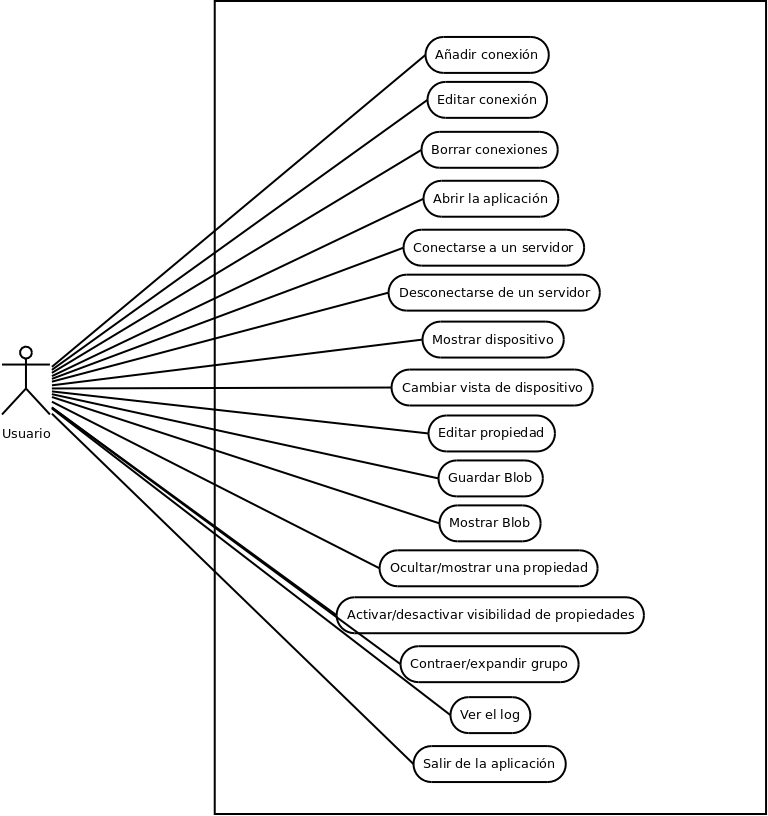
\includegraphics[width=1\textwidth]{../images/diagrama_casos_de_uso.png}
  \caption{Diagrama de casos de uso.}
  \label{fig:diag_scrum}
  \end{center}
\end{figure}